\documentclass[journal]{IEEEtran}

\usepackage{graphicx}
\usepackage{booktabs}
\usepackage{multirow}
\usepackage{array}
\usepackage{amsmath}
\usepackage{url}
\usepackage{cite}
\usepackage{siunitx}
\usepackage{xcolor}

\graphicspath{{figures/}}

\title{A Reproducible Comparative Evaluation of Swin-Tiny and ResNet-50 for Landfill-Candidate Classification in Aerial Imagery}

\author{Ashmit Iyer and Sarthak Sharma%
\thanks{The authors are with Kalinga Institute of Industrial Technology (KIIT), Bhubaneswar, India.}
}

\begin{document}
\maketitle

\begin{abstract}
Illegal landfill screening from aerial imagery can assist environmental monitoring by identifying locations that warrant further human inspection. This study presents a controlled comparative evaluation of a hierarchical vision transformer, Swin-Tiny, and a conventional convolutional neural network, ResNet-50, for binary landfill-candidate classification using the AerialWaste dataset. Both models were initialized with ImageNet-pretrained weights and evaluated under the same locked train-validation-test protocol, with model and decision-threshold selection restricted to validation data and the held-out test set reserved exclusively for final evaluation. On the 2,607-image test set, Swin-Tiny achieved 92.60\% accuracy, 86.74\% precision, 91.83\% recall, 89.21\% F1-score, and 97.84\% ROC-AUC, while ResNet-50 achieved 91.94\%, 87.74\%, 88.15\%, 87.94\%, and 97.13\%, respectively. Bootstrap confidence intervals quantified uncertainty, while an exact paired McNemar test yielded $p=0.2518$, indicating that the observed difference in paired classification correctness was not statistically significant. Swin-Tiny also made fewer errors on candidate-location images, whereas ResNet-50 showed substantially lower inference latency. On a Tesla T4 GPU at $224\times224$ input resolution, mean latency was 4.651 ms per image for Swin-Tiny and 3.047 ms for ResNet-50, with ResNet-50 achieving approximately 1.53$\times$ the throughput of Swin-Tiny. Calibration metrics were similar between the models. Overall, the results characterize a performance-efficiency trade-off and illustrate the value of controlled evaluation, uncertainty estimation, error analysis, and computational benchmarking for aerial landfill screening.
\end{abstract}

\begin{IEEEkeywords}
aerial imagery, landfill detection, remote sensing, Swin Transformer, ResNet-50, image classification, AerialWaste, deep learning
\end{IEEEkeywords}

\section{Introduction}
Illegal waste dumping and uncontrolled disposal sites pose environmental risks and require monitoring by environmental authorities. Identifying potentially problematic sites over large geographic regions is challenging because conventional inspection relies substantially on manual interpretation of aerial imagery and expert knowledge. The increasing availability of high-resolution aerial and satellite imagery provides an opportunity to automate part of this screening process using computer vision and deep learning.

The development of such systems depends strongly on representative and professionally annotated datasets. The AerialWaste dataset was introduced to support landfill discovery from aerial and satellite imagery and contains binary annotations together with metadata describing characteristics of positive sites \cite{torres2023aerialwaste}. The original dataset publication reports 10,434 images from Lombardy, Italy, comprising 3,478 positive and 6,956 negative examples \cite{torres2023aerialwaste}.

The original AerialWaste technical-validation study formulated illegal-landfill discovery as a scene-classification problem and used a ResNet-50-based architecture with feature-pyramid connections \cite{torres2021illegal}. This work established the feasibility of learning landfill-related visual patterns from aerial imagery.

However, comparisons between published AerialWaste studies are difficult because experimental protocols differ in dataset partitioning, model initialization, image resolution, fine-tuning strategy, augmentation, classification heads, and evaluation methodology. Consequently, differences in reported performance cannot necessarily be attributed to architecture alone \cite{gibellini2025pipeline,sharmily2025landfill,anvith2026secbam}.

This study addresses this issue through a controlled comparative evaluation of Swin-Tiny and ResNet-50 on a fixed train-validation-test partition of AerialWaste. Both models are initialized using ImageNet-pretrained weights and evaluated at the same input resolution under a common experimental protocol. Model selection and decision-threshold selection are restricted to validation data, while the test set remains untouched until final evaluation.

Beyond conventional classification metrics, the study evaluates the two architectures using bootstrap confidence intervals, paired statistical testing, probability calibration, inference efficiency, and structured error analysis. Bootstrap confidence intervals are used to quantify sampling uncertainty \cite{efron1993bootstrap}, while paired McNemar testing evaluates differences in correctness on the same test instances \cite{dietterich1998tests}. Calibration is assessed using expected calibration error and Brier score \cite{guo2017calibration}, and inference efficiency is measured under a controlled GPU benchmark.

The main contributions are: (1) a controlled Swin-Tiny versus ResNet-50 comparison using the same locked AerialWaste protocol; (2) uncertainty-aware evaluation using bootstrap confidence intervals and paired McNemar testing; (3) calibration and GPU inference-efficiency analysis; (4) structured analysis of shared and model-specific errors; and (5) characterization of the predictive-performance and computational-efficiency trade-off between the two architectures. These contributions are empirical and methodological; the study does not claim a new architecture or universal superiority of either model.

\section{Related Work}
\subsection{Deep Learning for Aerial Waste Detection}
Torres and Fraternali introduced AerialWaste to support automated landfill discovery using professionally interpreted aerial and satellite imagery \cite{torres2023aerialwaste}. The dataset provides binary landfill annotations together with metadata describing properties such as evidence, severity, site type, and visible waste characteristics \cite{torres2023aerialwaste}.

Torres and Fraternali formulated illegal-landfill discovery as a multi-scale scene-classification problem and used a ResNet-50 architecture augmented with feature-pyramid connections \cite{torres2021illegal}. Their results demonstrated the feasibility of CNN-based scene classification for this application.

\subsection{CNN-Based Approaches}
Convolutional neural networks remain widely used for remote-sensing image classification because hierarchical feature representations can capture spatial structure at multiple scales. In the AerialWaste literature, CNN-based and lightweight approaches have been investigated alongside more recent transformer-based models \cite{torres2021illegal,gibellini2025pipeline,sharmily2025landfill}.

\subsection{Vision Transformers}
Vision transformers provide an alternative to convolutional architectures by modeling relationships between image regions using self-attention. The Vision Transformer demonstrated the applicability of transformer architectures to image recognition at scale \cite{dosovitskiy2021vit}, while Swin Transformer introduced hierarchical representations and shifted local attention windows to improve computational scalability \cite{liu2021swin}. ResNet architectures provide a strong convolutional reference point for image recognition \cite{he2016resnet}.

Recent AerialWaste research has evaluated both transformer and attention-enhanced architectures. Gibellini et al. reported a best configuration with 92.02\% F1-score and 94.56\% accuracy and also examined generalization to visually different territories \cite{gibellini2025pipeline}. Sharmily et al. reported 92.41\% F1-score using an ensemble of lightweight architectures \cite{sharmily2025landfill}. A 2026 study evaluated frozen ResNet-50 and other CNN/transformer baselines and proposed an attention-enhanced ViT-based model, reporting 93.06\% accuracy and 90.09\% balanced F1-score for its proposed method \cite{anvith2026secbam}. These results demonstrate active interest in AerialWaste, but the differing subsets, preprocessing, training protocols, and evaluation designs prevent direct numerical ranking against the present study.

\subsection{Research Gap}
Existing AerialWaste studies demonstrate strong performance across conventional CNN, lightweight, and transformer architectures \cite{torres2021illegal,gibellini2025pipeline,sharmily2025landfill,anvith2026secbam}. The present study therefore focuses on controlled comparative evaluation rather than architectural novelty: the dataset partition, input resolution, model-selection rule, and held-out test set are fixed, while uncertainty, paired testing, calibration, computational efficiency, and structured error behavior are reported explicitly.

\section{Dataset and Experimental Protocol}
\subsection{Dataset}
The experiments used AerialWaste v3.0 for binary image-level classification of landfill candidates and non-candidates. The working dataset contained 11,703 unique PNG images, comprising 9,096 images from the training manifest and 2,607 images from the original testing manifest. The training manifest contained 6,064 class-0 images and 3,032 class-1 images, while the held-out testing manifest contained 1,738 class-0 and 869 class-1 images. No filename overlap was observed between the training and testing manifests. The approximately 11,700-image Version 3 release is also described in recent AerialWaste research \cite{gibellini2025pipeline}. The overall experimental workflow is summarized in Fig.~\ref{fig:workflow}.

\begin{figure}[t]
\centering
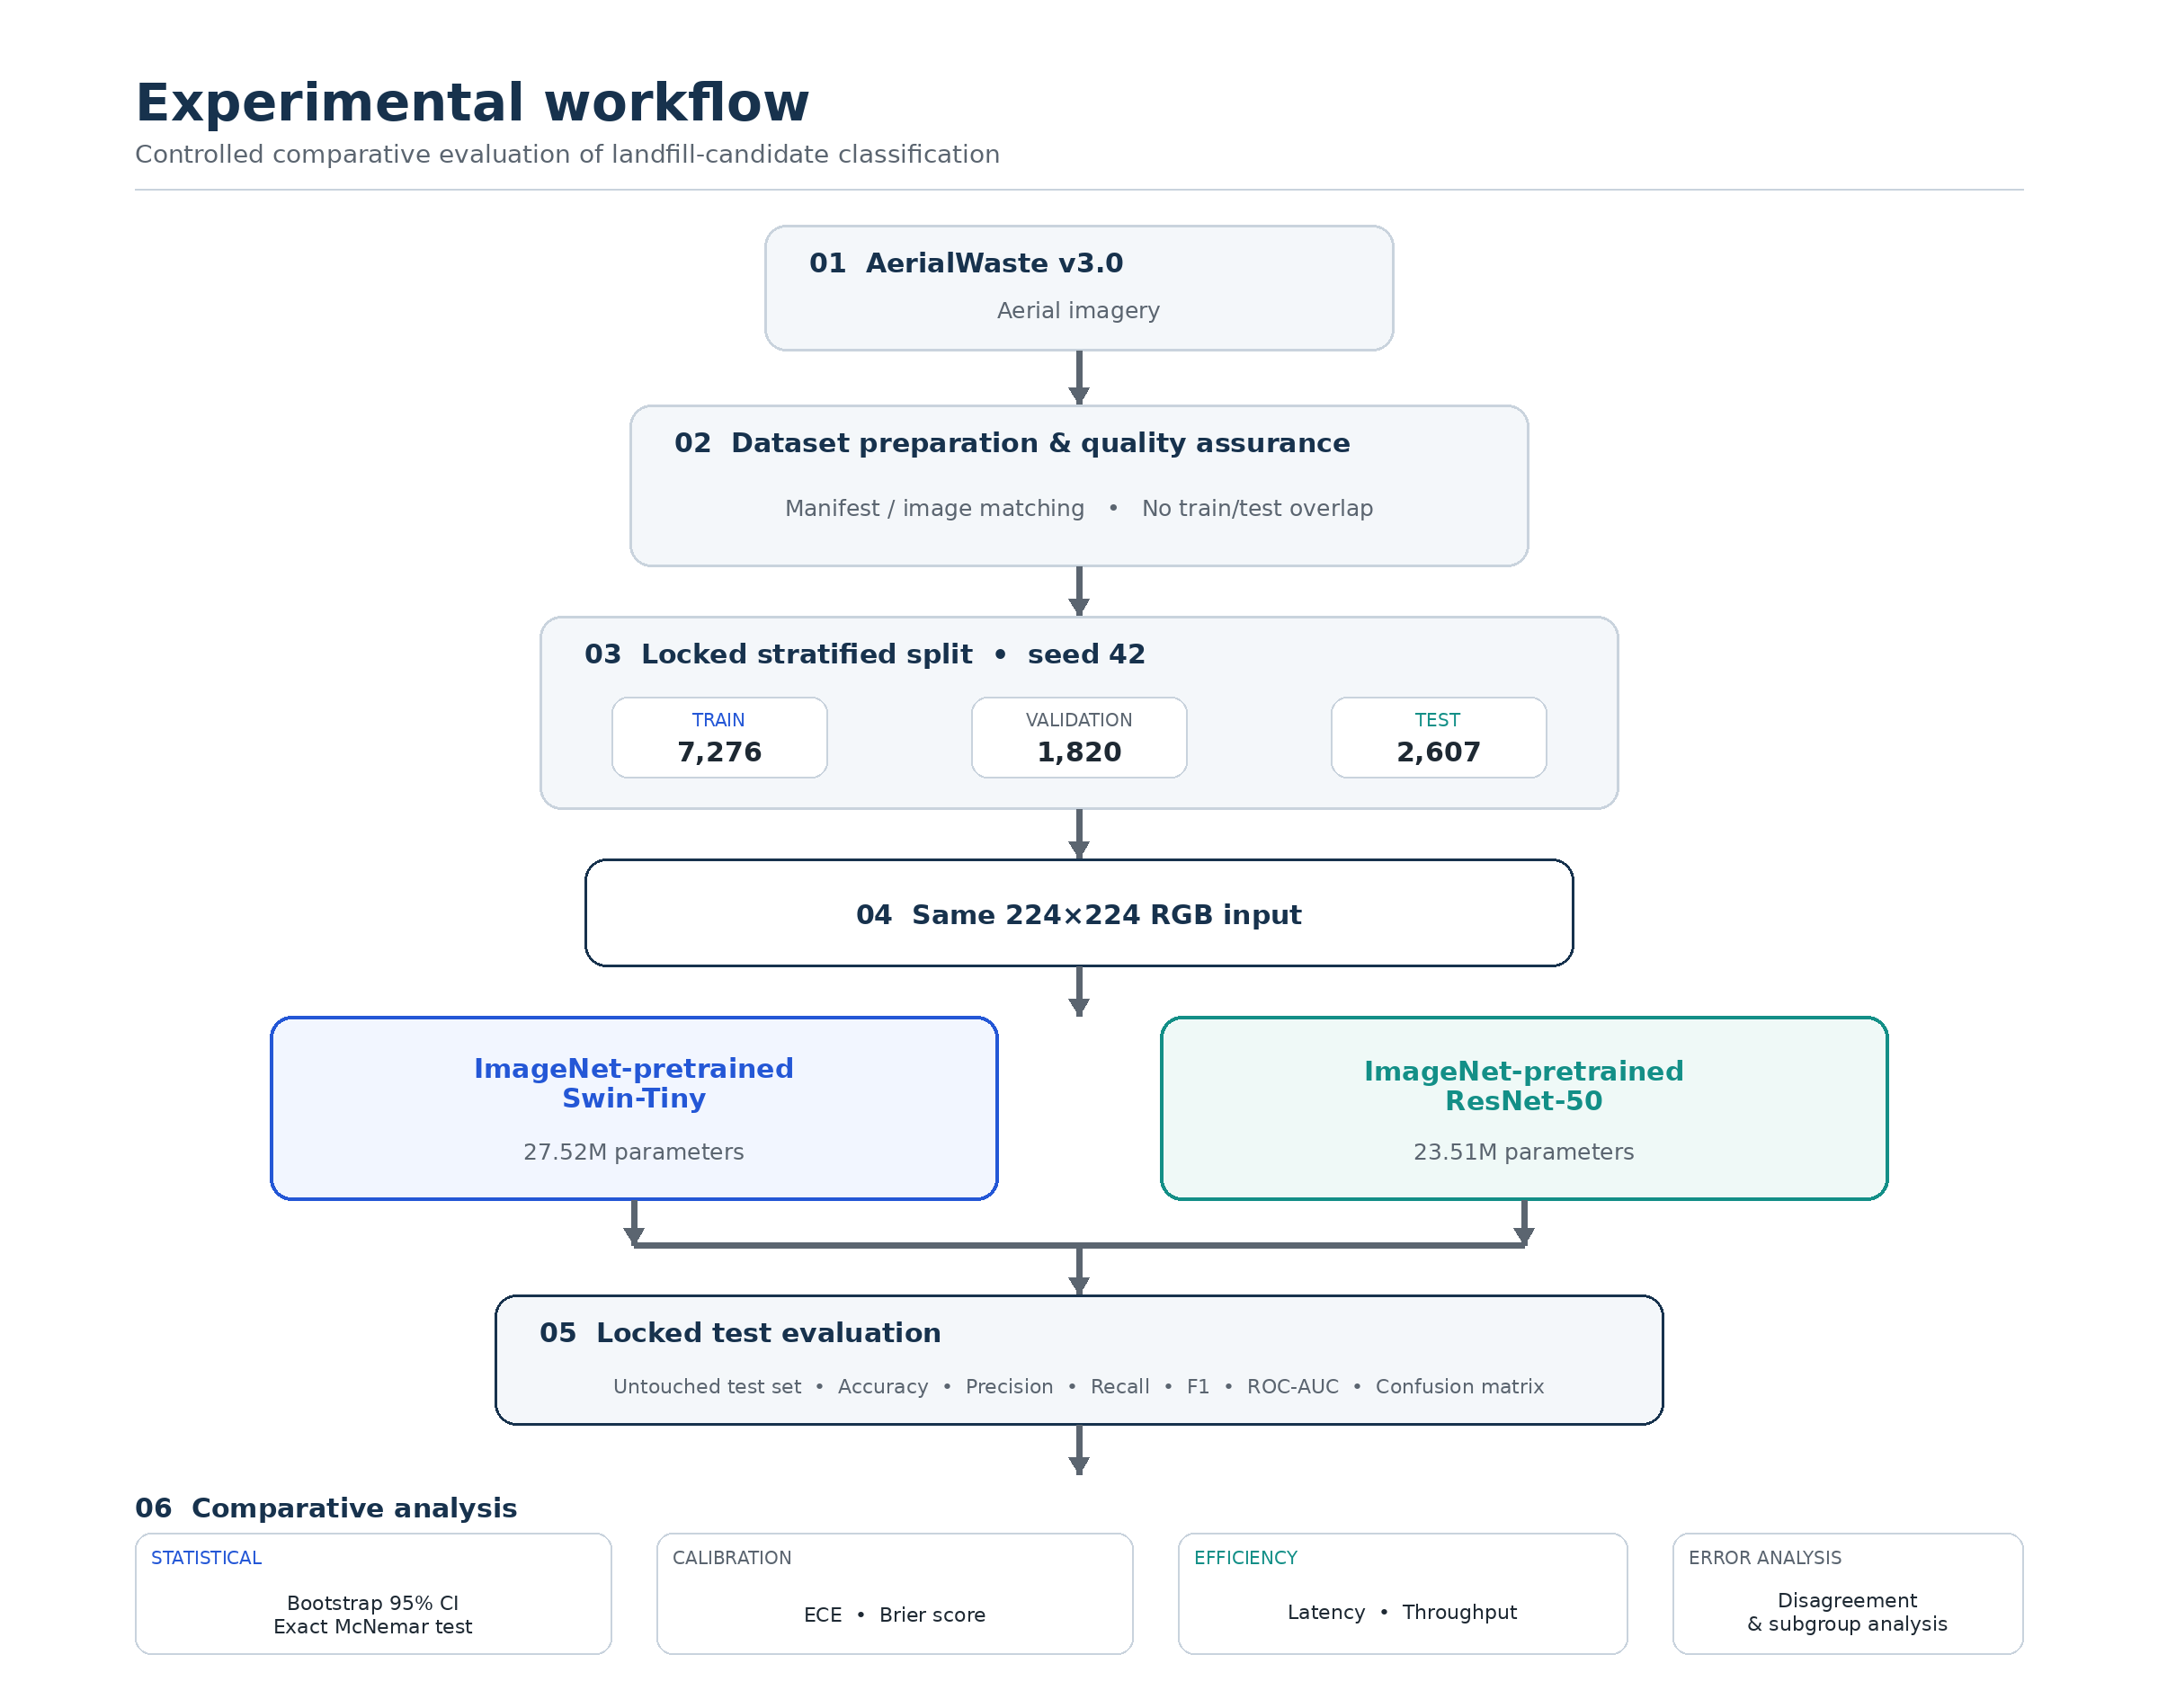
\includegraphics[width=\columnwidth]{Fig1_Experimental_Workflow_Final.png}
\caption{Experimental workflow for the controlled comparative evaluation.}
\label{fig:workflow}
\end{figure}

Manifest-based filename matching was used to verify image availability. A random read test of 100 images was successful. A complete decode audit of all 11,703 images was not completed; therefore, exhaustive pixel-level validation of every image is not claimed.

\subsection{Locked Train-Validation-Test Split}
The original training manifest was divided into training and validation subsets using a stratified 80:20 split with random seed 42. The original testing manifest was retained completely as the independent held-out test set.

The three split manifests were fixed and reused throughout the experiments. Split-overlap checks confirmed no overlapping filenames, and missing-image checks returned zero missing files. The test set was not used for model selection, hyperparameter tuning, threshold selection, or checkpoint selection.

\begin{table}[t]
\caption{Locked dataset split.}
\label{tab:split}
\centering
\begin{tabular}{lrrr}
\toprule
Split & Total & Class 0 & Class 1\\
\midrule
Training & 7,276 & 4,851 & 2,425\\
Validation & 1,820 & 1,213 & 607\\
Test & 2,607 & 1,738 & 869\\
Total & 11,703 & 7,802 & 3,901\\
\bottomrule
\end{tabular}
\end{table}

\subsection{Image Preprocessing}
Both architectures used a common input resolution of $224\times224$ pixels and ImageNet-pretrained initialization. ImageNet pretraining is based on the large-scale ImageNet recognition benchmark \cite{krizhevsky2012imagenet,deng2009imagenet}. Each classification head was configured for the two-class candidate/non-candidate task.

\subsection{Model Architectures}
The transformer-based model was Swin-Tiny (\texttt{swin\_tiny\_patch4\_window7\_224}), containing 27,520,892 parameters \cite{liu2021swin}. The convolutional baseline was ImageNet-pretrained ResNet-50, containing 23,512,130 parameters in the experimental configuration \cite{he2016resnet}.

\subsection{Training Protocol}
ResNet-50 used batch size 16, maximum 11 epochs, stochastic gradient descent with learning rate 0.001, momentum 0.9, weight decay $10^{-4}$, CUDA automatic mixed precision, and early stopping with validation F1 as the checkpoint-selection metric. Swin-Tiny was likewise selected using validation F1, with the best validation F1 of approximately 0.8954 occurring at epoch 4 and early stopping after epoch 9.

\subsection{Decision Threshold Selection}
Decision thresholds were selected without using the held-out test set. Swin-Tiny used the validation-selected threshold of 0.45. ResNet-50 was evaluated at a threshold of 0.50.

\subsection{Evaluation Metrics}
Performance was evaluated using accuracy, precision, recall, F1-score, and ROC-AUC \cite{fawcett2006roc}. In addition, 95\% bootstrap confidence intervals \cite{efron1993bootstrap}, exact paired McNemar testing \cite{dietterich1998tests}, expected calibration error and Brier score \cite{guo2017calibration}, inference latency, throughput, and structured metadata-based error analysis were performed.

\section{Results}
\subsection{Overall Classification Performance}
Swin-Tiny achieved higher point estimates for accuracy, recall, F1-score, and ROC-AUC, whereas ResNet-50 achieved slightly higher precision. Swin-Tiny produced 122 false positives and 71 false negatives, while ResNet-50 produced 107 false positives and 103 false negatives. Thus, the point-estimate difference is characterized primarily by fewer false negatives for Swin-Tiny alongside slightly more false positives. The complete metric and confusion-matrix comparison is shown in Fig.~\ref{fig:performance}.

\begin{table}[t]
\caption{Held-out test performance.}
\label{tab:main}
\centering
\begin{tabular}{lcc}
\toprule
Metric & Swin-Tiny & ResNet-50\\
\midrule
Accuracy & 92.60\% & 91.94\%\\
Precision & 86.74\% & 87.74\%\\
Recall & 91.83\% & 88.15\%\\
F1-score & 89.21\% & 87.94\%\\
ROC-AUC & 97.84\% & 97.13\%\\
\bottomrule
\end{tabular}
\end{table}

\begin{figure}[t]
\centering
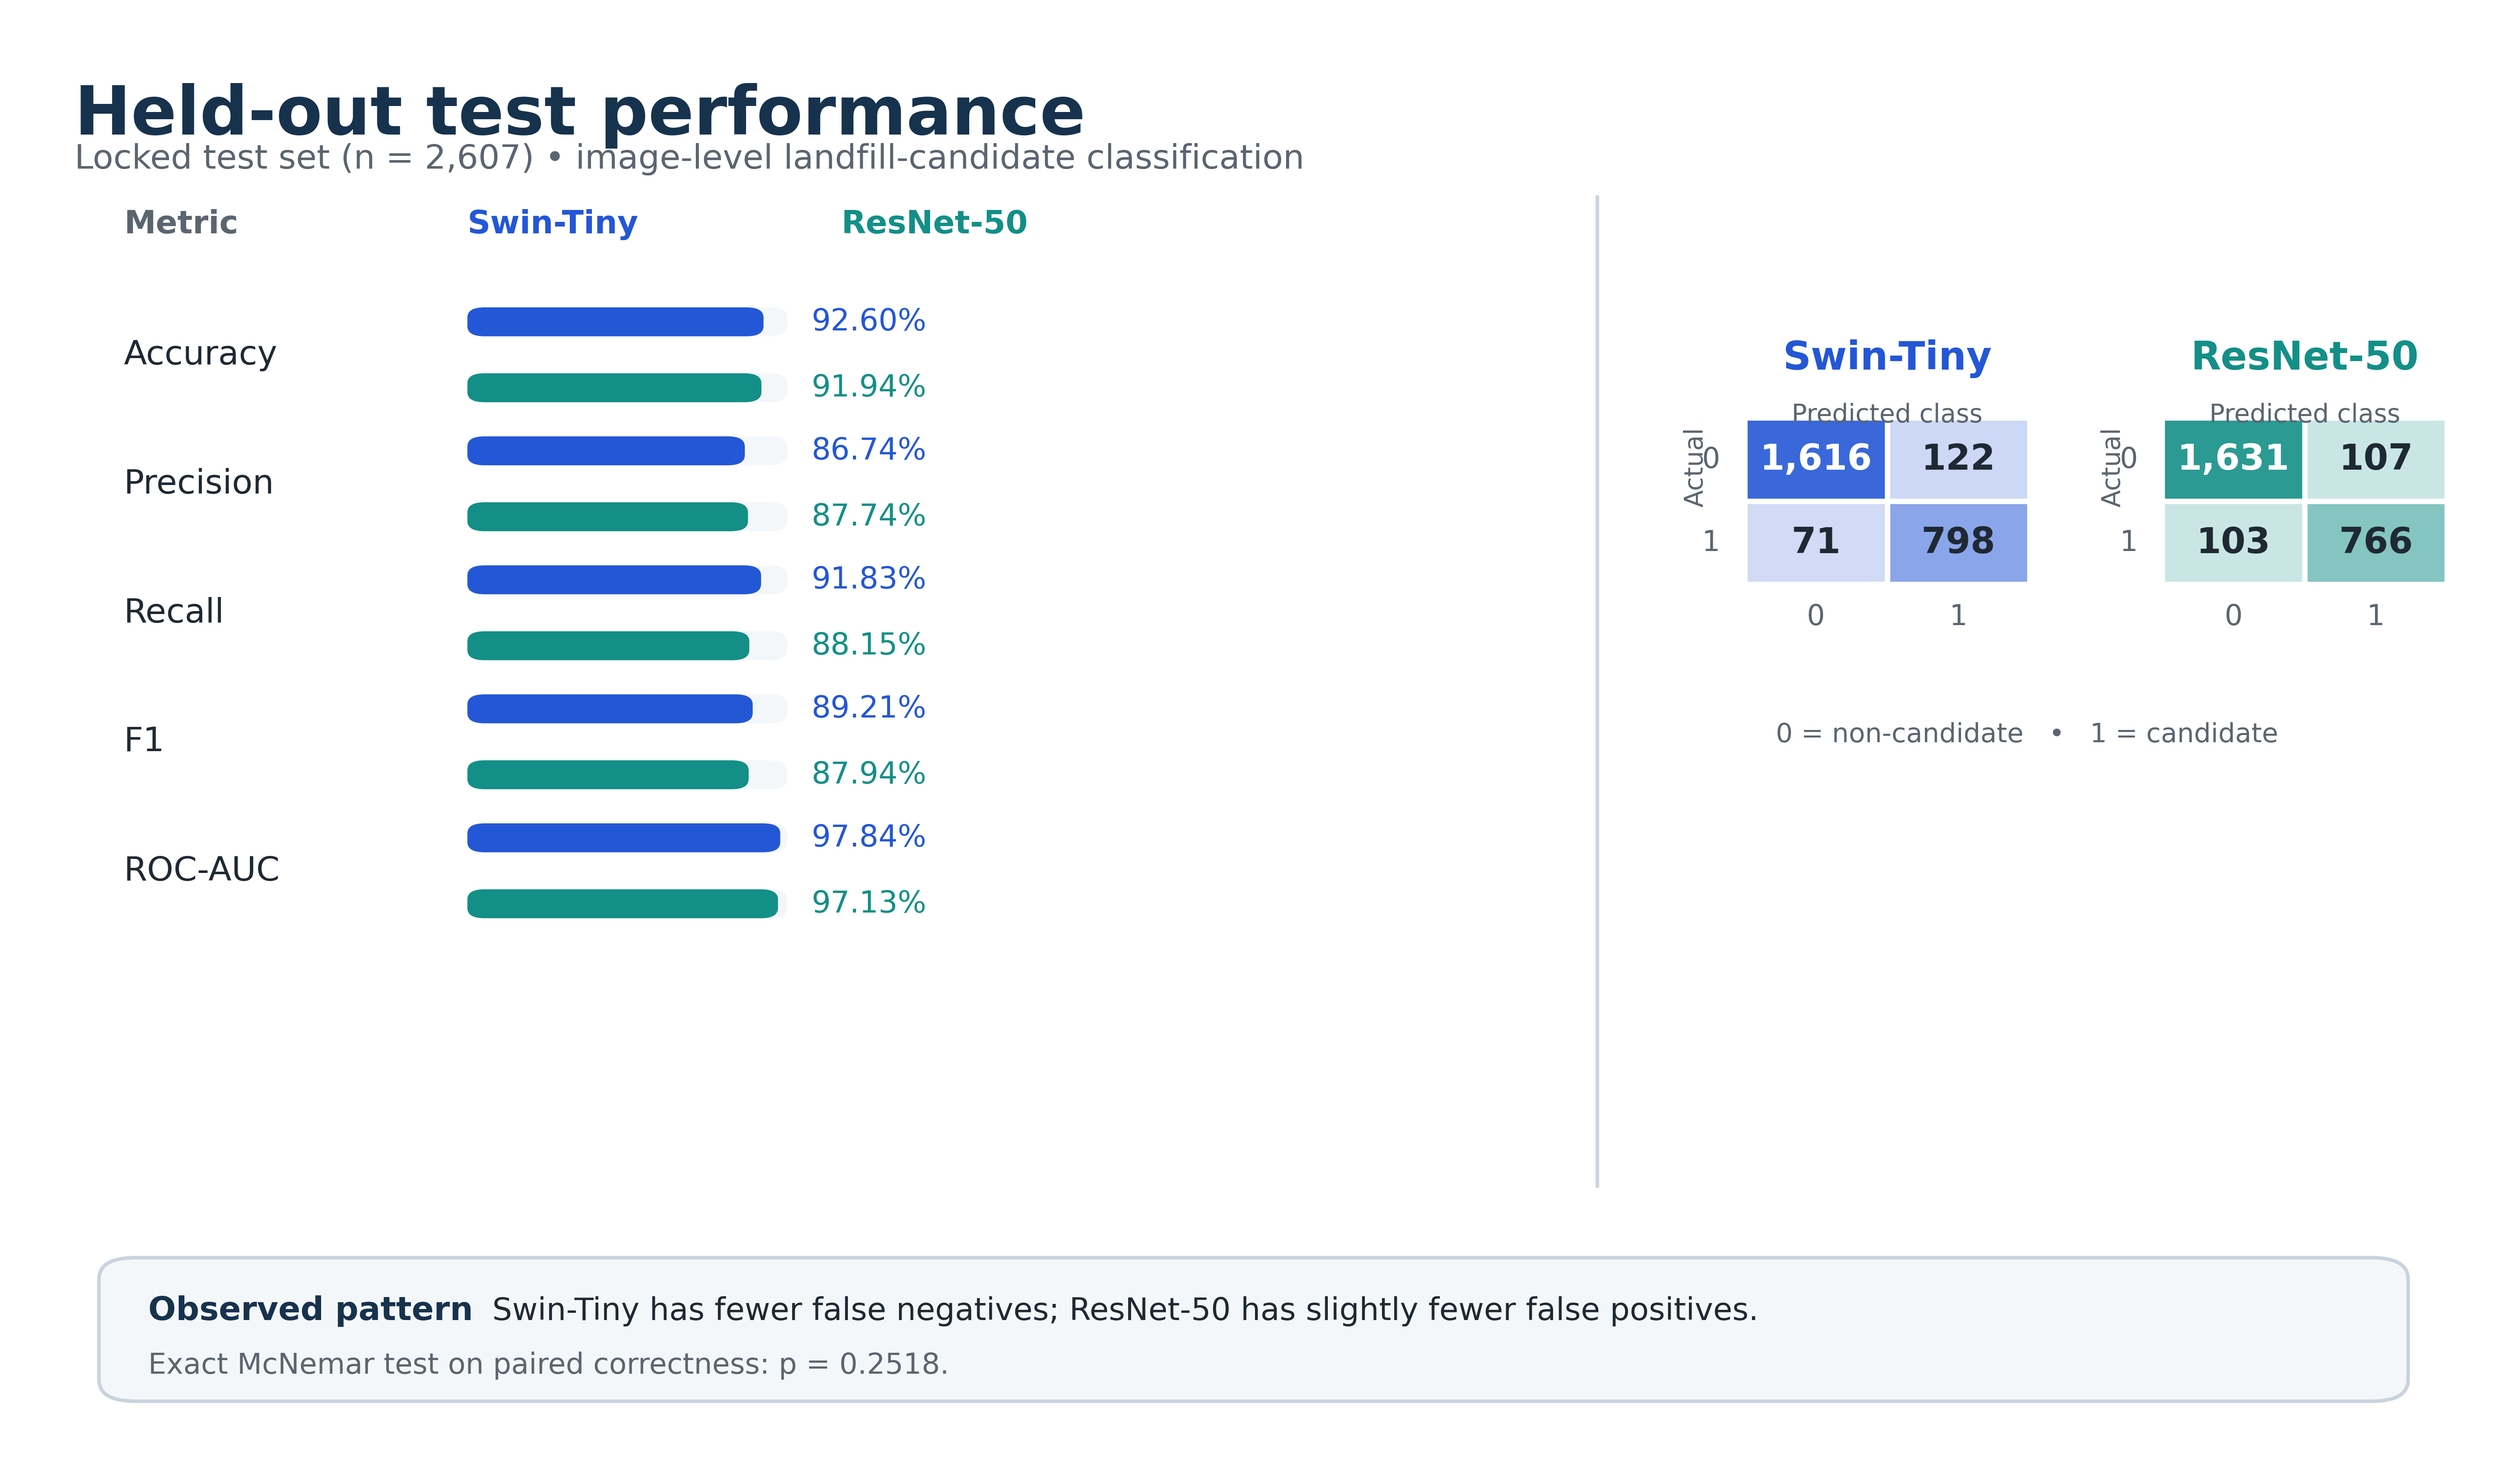
\includegraphics[width=\columnwidth]{Fig2_Performance_Confusion_Final.png}
\caption{Held-out test performance and confusion matrices for Swin-Tiny and ResNet-50.}
\label{fig:performance}
\end{figure}

\subsection{Statistical Comparison}
The models agreed on correctness for 2,412 of 2,607 images (92.52\%). The exact McNemar test yielded $p=0.2518$. Thus, the observed difference in paired classification correctness was not statistically significant, and the point-estimate differences should not be interpreted as evidence of overall architectural superiority.

\begin{table}[t]
\caption{Paired prediction correctness on the locked test set.}
\label{tab:mcnemar}
\centering
\begin{tabular}{lrr}
\toprule
Prediction outcome & Images & Percentage\\
\midrule
Both correct & 2,308 & 88.53\%\\
Swin correct, R50 incorrect & 106 & 4.07\%\\
R50 correct, Swin incorrect & 89 & 3.41\%\\
Both incorrect & 104 & 3.99\%\\
Total & 2,607 & 100.00\%\\
\bottomrule
\end{tabular}
\end{table}

\subsection{Bootstrap Confidence Intervals}
Bootstrap 95\% confidence intervals for all five metrics are shown in Fig.~\ref{fig:bootstrap}. The intervals quantify uncertainty around the point estimates reported in Table~\ref{tab:ci}; they are descriptive intervals and are not, by themselves, a formal paired significance test.

\begin{table}[t]
\caption{Bootstrap 95\% confidence intervals.}
\label{tab:ci}
\centering
\begin{tabular}{lccrc}
\toprule
Metric & Swin-Tiny & 95\% CI & ResNet-50 & 95\% CI\\
\midrule
Accuracy & 92.60\% & [91.60, 93.59] & 91.94\% & [90.91, 92.98]\\
Precision & 86.74\% & [84.55, 88.88] & 87.74\% & [85.50, 89.86]\\
Recall & 91.83\% & [89.99, 93.57] & 88.15\% & [85.96, 90.24]\\
F1-score & 89.21\% & [87.69, 90.71] & 87.94\% & [86.28, 89.50]\\
ROC-AUC & 97.84\% & [97.37, 98.28] & 97.13\% & [96.56, 97.67]\\
\bottomrule
\end{tabular}
\end{table}

\begin{figure}[t]
\centering
\includegraphics[width=\columnwidth]{Fig5_Bootstrap_CI_Final.png}
\caption{Bootstrap 95\% confidence intervals for test-set performance metrics.}
\label{fig:bootstrap}
\end{figure}

\subsection{Calibration}
Swin-Tiny exhibited slightly lower ECE and Brier score. These differences are descriptive because no statistical significance test was performed for calibration; the results therefore support a statement of similar calibration behavior rather than a claim of statistically better calibration.

\begin{table}[t]
\caption{Calibration metrics.}
\label{tab:calibration}
\centering
\begin{tabular}{lcc}
\toprule
Metric & Swin-Tiny & ResNet-50\\
\midrule
ECE & 0.0286 & 0.0293\\
Brier score & 0.0553 & 0.0609\\
\bottomrule
\end{tabular}
\end{table}

\subsection{Inference Efficiency}
ResNet-50 required approximately 1.53$\times$ less inference time per image and achieved approximately 1.53$\times$ higher throughput under the Tesla T4 benchmark conditions. The performance-efficiency relationship is visualized in Fig.~\ref{fig:efficiency}. These measurements exclude data loading and preprocessing and should be interpreted as hardware- and software-configuration-specific.

\begin{table}[t]
\caption{Inference efficiency.}
\label{tab:efficiency}
\centering
\begin{tabular}{lcc}
\toprule
Metric & Swin-Tiny & ResNet-50\\
\midrule
Parameters & 27.52M & 23.51M\\
Mean latency/image & 4.651 $\pm$ 0.106 ms & 3.047 $\pm$ 0.030 ms\\
Median latency/image & 4.634 ms & 3.042 ms\\
Mean throughput & 215.1 $\pm$ 4.8 img/s & 328.3 $\pm$ 3.2 img/s\\
Median throughput & 215.8 img/s & 328.7 img/s\\
\bottomrule
\end{tabular}
\end{table}

\begin{figure}[t]
\centering
\includegraphics[width=\columnwidth]{Fig3_Performance_Efficiency_Final.png}
\caption{Predictive performance versus inference efficiency under the interleaved Tesla T4 benchmark.}
\label{fig:efficiency}
\end{figure}

\subsection{Error Analysis}
Overall model disagreement occurred on 195 images (7.48\%). Swin-Tiny was correct on 106 images for which ResNet-50 was incorrect, whereas ResNet-50 was correct on 89 images for which Swin-Tiny was incorrect. Fig.~\ref{fig:error} summarizes the paired error decomposition and the candidate-location subgroup. The directional difference is descriptive because the paired McNemar test did not reach statistical significance.

\begin{figure}[t]
\centering
\includegraphics[width=\columnwidth]{Fig4_Error_Analysis_Final.png}
\caption{Paired prediction agreement and error rates by true class on the locked test set.}
\label{fig:error}
\end{figure}

\subsection{Metadata-Based Error Analysis}
Among candidate-location images, Swin-Tiny produced 71 errors compared with 103 for ResNet-50, corresponding to error rates of 8.17\% and 11.85\%, respectively. This subgroup pattern is consistent with the higher candidate-class recall of Swin-Tiny. Other metadata categories showed variable error rates, but several subgroups were small or contained unspecified values; these analyses are therefore treated as descriptive. A qualitative visual inspection of selected errors could not be completed because the corresponding image files were unavailable in the analysis runtime.

\begin{table}[t]
\caption{Error rates by true class.}
\label{tab:classerrors}
\centering
\begin{tabular}{lrrrrr}
\toprule
True class & $N$ & Swin errors & Swin rate & R50 errors & R50 rate\\
\midrule
Non-candidate & 1,738 & 122 & 7.02\% & 107 & 6.16\%\\
Candidate & 869 & 71 & 8.17\% & 103 & 11.85\%\\
\bottomrule
\end{tabular}
\end{table}


\section{Representative TP, TN, FP, and FN Cases}

The following examples provide a qualitative view of the four possible prediction outcomes on the held-out AerialWaste test set. True-positive and true-negative examples correspond to correct candidate and non-candidate predictions, respectively. False-positive examples show non-candidate images that were classified as candidates, while false-negative examples show candidate images that were classified as non-candidates. The figure reports representative predictions from both Swin-Tiny and ResNet-50 together with the associated confidence values.

\begin{figure*}[!t]
\centering
\includegraphics[width=0.92\textwidth]{Fig6_Representative_TP_TN_FP_FN_AerialWaste.png}
\caption{Representative true-positive, true-negative, false-positive, and false-negative predictions on the held-out AerialWaste test set for Swin-Tiny and ResNet-50.}
\label{fig:representative_errors}
\end{figure*}

The examples illustrate why image-level landfill-candidate screening remains challenging. Correct predictions can arise from scenes with substantial contextual cues, whereas false positives may be produced by visually complex terrain or structures that resemble candidate locations. False negatives are particularly relevant for screening applications because visually ambiguous candidate sites may be overlooked. These examples are qualitative and are intended to complement the aggregate error statistics rather than replace them.

\section{Discussion}
\subsection{Comparative Model Performance}
Both models provided strong classification performance under the locked protocol. Swin-Tiny obtained higher point estimates for accuracy, recall, F1-score, and ROC-AUC, while ResNet-50 achieved slightly higher precision. The recall difference corresponds to fewer false negatives for Swin-Tiny but more false positives. Because the exact McNemar test was not significant, these differences should be interpreted as empirical point-estimate differences rather than statistically established architectural superiority.

\subsection{Comparison With Previous AerialWaste Studies}
Recent AerialWaste studies have reported strong performance using CNN, lightweight, and transformer-based approaches \cite{gibellini2025pipeline,sharmily2025landfill,anvith2026secbam}. These studies are informative context but are not directly comparable to the present results because they use different data subsets, preprocessing, training procedures, model-selection strategies, and evaluation protocols. In particular, Gibellini et al. reported 92.02\% F1-score and 94.56\% accuracy for their best configuration and also evaluated cross-territory generalization \cite{gibellini2025pipeline}, while Sharmily et al. reported 92.41\% F1-score for a lightweight-model ensemble \cite{sharmily2025landfill}. A 2026 study reported 93.06\% accuracy and 90.09\% balanced F1-score for an attention-enhanced ViT-based model \cite{anvith2026secbam}. These values should be viewed as contextual evidence of activity on AerialWaste rather than as a common leaderboard.

\subsection{Performance-Efficiency Trade-off}
The predictive and computational results demonstrate a practical trade-off. Swin-Tiny showed higher point estimates for several predictive metrics, whereas ResNet-50 provided lower latency and higher throughput. Deployment decisions should therefore consider both predictive requirements and computational constraints.

\subsection{Candidate-Location Error Behavior}
The candidate-location subgroup showed 71 Swin-Tiny errors versus 103 ResNet-50 errors, corresponding to error rates of 8.17\% versus 11.85\%. This pattern is consistent with the higher candidate-class recall of Swin-Tiny, but it remains a descriptive observation from one held-out test set and was not separately subjected to a multiplicity-adjusted significance test.

\subsection{Calibration and Confidence}
Calibration metrics were similar between models, with ECE values of 0.0286 and 0.0293 and Brier scores of 0.0553 and 0.0609 for Swin-Tiny and ResNet-50, respectively. Both models also produced some highly confident incorrect predictions, demonstrating that confidence should not be treated as proof of correctness in environmental screening.

\subsection{Implications for Environmental Screening}
The classifier is best viewed as a candidate-screening component that can prioritize imagery for subsequent human inspection. A positive prediction does not establish illegal activity, and the appropriate operating threshold would ultimately depend on deployment-specific costs of missed candidates and unnecessary inspections.

\subsection{Reproducibility as a Contribution}
The study's methodological contribution is the controlled evaluation protocol: identical locked partitions, common input resolution, validation-only model and threshold selection, untouched test data, paired statistical testing, calibration assessment, efficiency measurement, and structured error analysis. The resulting comparison is intended as a reproducible empirical study rather than a claim of a new model architecture.

\section{Limitations}
The task is image-level candidate classification rather than direct legal or field verification of illegal activity.

The experiments use one locked test release and one random training-validation split and therefore do not establish geographic or sensor-independent generalization.

The dataset has a geographically specific origin, so results should not automatically be generalized to other regions, sensors, or acquisition conditions.

The McNemar test was based on one paired test set and did not establish a statistically significant overall correctness difference.

Metadata subgroups are unevenly distributed and some contain unspecified values, limiting inferential interpretation.

Selected qualitative visual error inspection could not be completed because the corresponding image files were unavailable in the analysis runtime.

Inference efficiency was measured on a Tesla T4 GPU and is therefore hardware- and software-configuration-specific.

\section{Conclusion}
This study presented a controlled comparative evaluation of Swin-Tiny and ResNet-50 for binary landfill-candidate classification in aerial imagery using AerialWaste. Under an identical locked evaluation protocol, Swin-Tiny achieved higher point estimates for accuracy, recall, F1-score, and ROC-AUC, while ResNet-50 achieved slightly higher precision and substantially lower inference latency. The exact paired McNemar test did not identify a statistically significant difference in overall classification correctness. The candidate-location analysis showed fewer errors for Swin-Tiny, while the efficiency benchmark showed substantially higher throughput for ResNet-50. These results characterize a performance-efficiency trade-off rather than universal superiority of one architecture. The study's conclusions are limited to the locked AerialWaste test release and the experimental conditions reported here; future work should test whether the observed patterns persist under genuinely held-out geographic or sensor domains.

\section*{Data Availability}
The AerialWaste Version 3 dataset used for this study is publicly distributed as part of the AerialWaste release described in recent work \cite{gibellini2025pipeline}. The present analysis uses the locked manifests and test release specified in Section III-A.


\begin{thebibliography}{14}

\bibitem{torres2023aerialwaste}
R. N. Torres and P. Fraternali, ``AerialWaste dataset for landfill discovery in aerial and satellite images,'' \emph{Scientific Data}, vol. 10, no. 1, p. 63, 2023, doi: 10.1038/s41597-023-01976-9.

\bibitem{torres2021illegal}
R. N. Torres and P. Fraternali, ``Learning to Identify Illegal Landfills through Scene Classification in Aerial Images,'' \emph{Remote Sensing}, vol. 13, no. 22, p. 4520, 2021, doi: 10.3390/rs13224520.

\bibitem{he2016resnet}
K. He, X. Zhang, S. Ren, and J. Sun, ``Deep Residual Learning for Image Recognition,'' in \emph{Proc. IEEE CVPR}, 2016, pp. 770--778, doi: 10.1109/CVPR.2016.90.

\bibitem{liu2021swin}
Z. Liu \emph{et al.}, ``Swin Transformer: Hierarchical Vision Transformer Using Shifted Windows,'' in \emph{Proc. IEEE/CVF ICCV}, 2021, pp. 10012--10022, doi: 10.1109/ICCV48922.2021.00986.

\bibitem{dosovitskiy2021vit}
A. Dosovitskiy \emph{et al.}, ``An Image is Worth 16x16 Words: Transformers for Image Recognition at Scale,'' in \emph{Proc. ICLR}, 2021.

\bibitem{guo2017calibration}
C. Guo, G. Pleiss, Y. Sun, and K. Q. Weinberger, ``On Calibration of Modern Neural Networks,'' in \emph{Proc. ICML}, vol. 70, 2017, pp. 1321--1330.

\bibitem{dietterich1998tests}
T. G. Dietterich, ``Approximate Statistical Tests for Comparing Supervised Classification Learning Algorithms,'' \emph{Neural Computation}, vol. 10, no. 7, pp. 1895--1923, 1998, doi: 10.1162/089976698300017197.

\bibitem{gibellini2025pipeline}
F. Gibellini \emph{et al.}, ``A Deep Learning Pipeline for Solid Waste Detection in Remote Sensing Images,'' \emph{Waste Management Bulletin}, vol. 3, no. 4, p. 100246, 2025, doi: 10.1016/j.wmb.2025.100246.

\bibitem{sharmily2025landfill}
N. Sharmily \emph{et al.}, ``Automated Landfill Detection Using Deep Learning: A Comparative Study of Lightweight and Custom Architectures with the AerialWaste Dataset,'' arXiv:2508.18315, 2025, doi: 10.48550/arXiv.2508.18315.

\bibitem{anvith2026secbam}
Anvith S. G., Nithish Kushal Reddy, and Rimjhim Padam Singh, ``SE-CBAM Augmented Vision Transformer and Imbalance-Aware Loss for High-Resolution Waste-Site Classification,'' \emph{Procedia Computer Science}, vol. 283, pp. 4061--4070, 2026, doi: 10.1016/j.procs.2026.06.467.

\bibitem{krizhevsky2012imagenet}
A. Krizhevsky, I. Sutskever, and G. E. Hinton, ``ImageNet classification with deep convolutional neural networks,'' in \emph{Advances in Neural Information Processing Systems}, 2012, pp. 1097--1105.

\bibitem{deng2009imagenet}
J. Deng \emph{et al.}, ``ImageNet: A Large-Scale Hierarchical Image Database,'' in \emph{Proc. IEEE CVPR}, 2009, pp. 248--255.

\bibitem{efron1993bootstrap}
B. Efron and R. J. Tibshirani, \emph{An Introduction to the Bootstrap}. New York, NY, USA: Chapman and Hall, 1993.

\bibitem{fawcett2006roc}
T. Fawcett, ``An introduction to ROC analysis,'' \emph{Pattern Recognition Letters}, vol. 27, no. 8, pp. 861--874, 2006, doi: 10.1016/j.patrec.2005.10.010.

\end{thebibliography}


\end{document}